% can't include for some reason... must be input
\pagebreak
\subsection{run\_AGC\_mod - WIP}
Sloppily copied from: \verb|200821-AGCicAdjTest|

uses Interchange modulation signal as perturbance

\textbf{AGC Modulation Test (Interchange adjustment) } \ \\

\begin{minipage}{0.5\linewidth}
\begin{itemize}
\raggedright
\item Event: When $t=5$ Area 2 increases its scheduled interchange by 0.2 PU.\\
Area 1 interchange is adjusted by -0.2 PU to keep system in balance.\\
Area 2 increases generation while Area 1 reduces generation.

\item Each area has non-conditional AGC set to act every 15 seconds and is forced to act by \verb|mAGC_sig| when the interchange adjustment first takes place.

%\item ODE solver tolerances:
%\subitem Relative: 1e-5
%\subitem Absolute: 1e-7
\end{itemize}
\vfill
\end{minipage}\hspace{2em}% 
\begin{minipage}{0.4\linewidth}
\centering
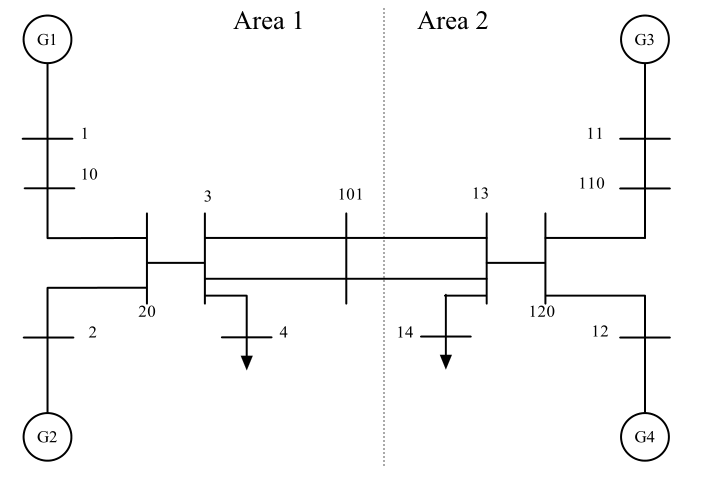
\includegraphics[width=\linewidth]{examples/agcMod/sysOneLineAreas}
\end{minipage}% 


\textbf{Result Summary:}
\begin{itemize}
\item Interchange adjustment seems to work correctly and is accounted for in AGC calculations.
\item The use of \verb|mAGC_sig| was tested as working using FTS or VTS.
\end{itemize}

\begin{minipage}{.5\linewidth}

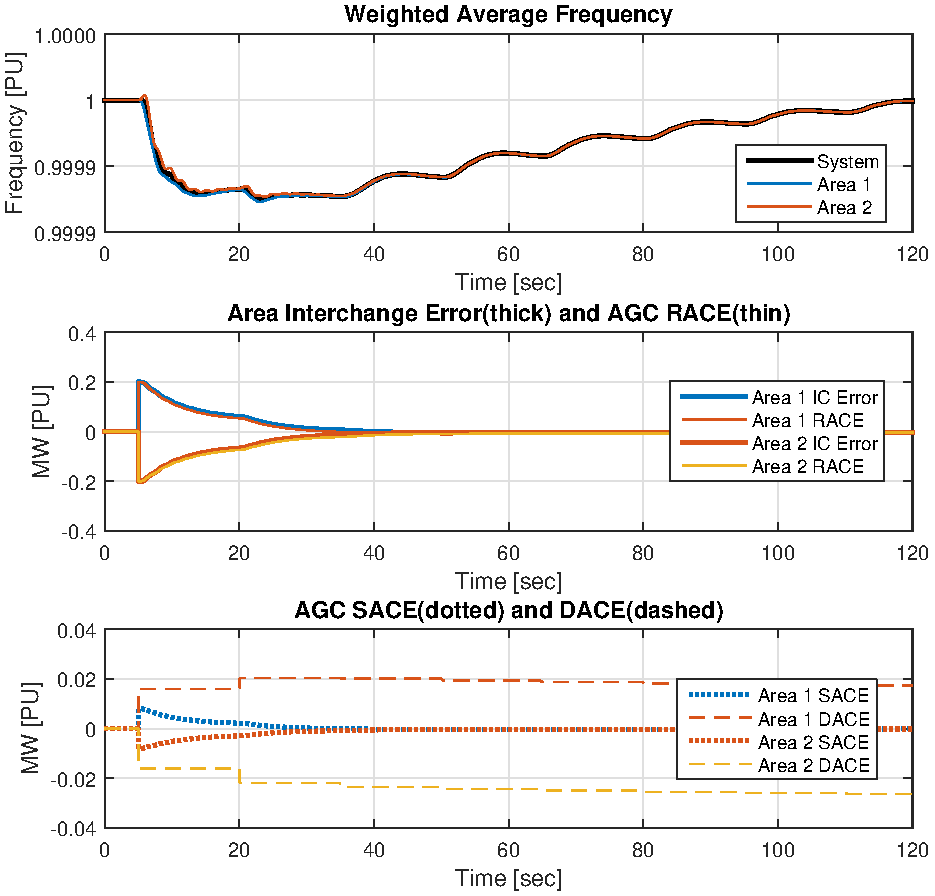
\includegraphics[width=\linewidth]{examples/agcMod/agcSigs}
\end{minipage}%
\begin{minipage}{.5\linewidth}

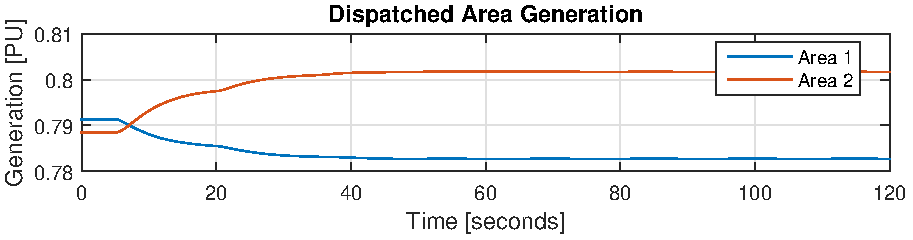
\includegraphics[width=\linewidth]{examples/agcMod/areaGen}

\vspace{1em}
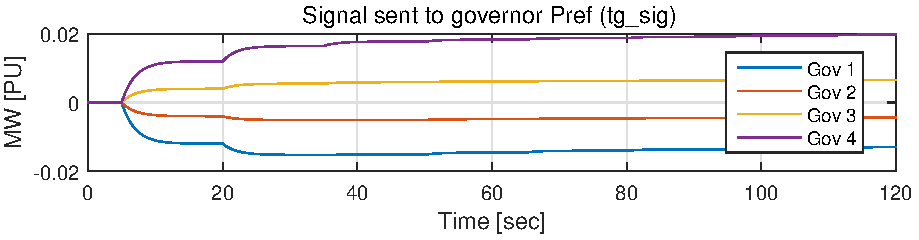
\includegraphics[width=\linewidth]{examples/agcMod/tgSigs}

\vspace{1em}
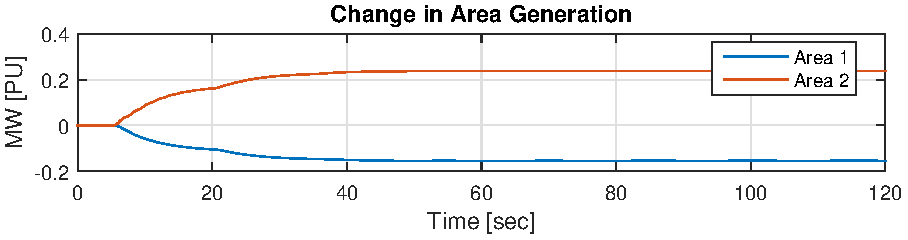
\includegraphics[width=\linewidth]{examples/agcMod/changeGen}
\end{minipage}

\textbf{Why this might matter: }
An extended term simulation may required the adjustment of scheduled interchange to achieve system recovery.
Specifically, if an area realizes that their available reserves become lower than was originally allocated for, a resolution may be to import more power from another area.
This added functionality will allow custom logic to handle such a scenario.

\pagebreak
\textbf{MATLAB modulation code} 
The \verb|mAGC_sig| file that adjusts the interchange and forces AGC action is shown below.


\begin{minted}[
		frame=lines,
		framesep=2mm,
		baselinestretch=1.2,
		bgcolor=gray!13,
		fontsize=\footnotesize,
		linenos,
		breaklines
		]{MATLAB}
function mAGC_sig(k)
% Syntax: mAGC_sig(k)
% input k is current data index
% 09:46 08/21/20
% place to define modulation signal for AGC operation

global g

%{
    Scenario:
Area 1 is exporting generation to Area 2 (Interchange value Positive)
Area 2 is importing power from Area 1 (Interchange value is Negative

Area 2 increases scheduled interchage, which reduces its scheduled import and causes area 2 to increase generation.
Area 1 decreases scheduled interchange to balance area 2 action.
As area 1 is exporting, the negative valued icAdj will reduce the generation in the area.

%}
persistent ForceDisptach

if g.sys.t(k) >= 5
    % adjust iterchange 
    g.area.area(2).icAdj(k) = 0.2;
    g.area.area(1).icAdj(k) = -0.2;
    
    % force AGC disptatch when interchange adjustment first applied
    if ForceDisptach
        g.agc.agc(1).nextActionTime = g.sys.t(k);
        g.agc.agc(2).nextActionTime = g.sys.t(k);
        ForceDisptach = 0;
    end
    
else
    g.area.area(2).icAdj(k) = 0;
    g.area.area(1).icAdj(k) = 0;
    ForceDisptach = 1;
end
end
\end{minted}
